% Options for packages loaded elsewhere
\PassOptionsToPackage{unicode}{hyperref}
\PassOptionsToPackage{hyphens}{url}
%
\documentclass[
]{article}
\usepackage{amsmath,amssymb}
\usepackage{iftex}
\ifPDFTeX
  \usepackage[T1]{fontenc}
  \usepackage[utf8]{inputenc}
  \usepackage{textcomp} % provide euro and other symbols
\else % if luatex or xetex
  \usepackage{unicode-math} % this also loads fontspec
  \defaultfontfeatures{Scale=MatchLowercase}
  \defaultfontfeatures[\rmfamily]{Ligatures=TeX,Scale=1}
\fi
\usepackage{lmodern}
\ifPDFTeX\else
  % xetex/luatex font selection
\fi
% Use upquote if available, for straight quotes in verbatim environments
\IfFileExists{upquote.sty}{\usepackage{upquote}}{}
\IfFileExists{microtype.sty}{% use microtype if available
  \usepackage[]{microtype}
  \UseMicrotypeSet[protrusion]{basicmath} % disable protrusion for tt fonts
}{}
\makeatletter
\@ifundefined{KOMAClassName}{% if non-KOMA class
  \IfFileExists{parskip.sty}{%
    \usepackage{parskip}
  }{% else
    \setlength{\parindent}{0pt}
    \setlength{\parskip}{6pt plus 2pt minus 1pt}}
}{% if KOMA class
  \KOMAoptions{parskip=half}}
\makeatother
\usepackage{xcolor}
\usepackage[margin=1in]{geometry}
\usepackage{color}
\usepackage{fancyvrb}
\newcommand{\VerbBar}{|}
\newcommand{\VERB}{\Verb[commandchars=\\\{\}]}
\DefineVerbatimEnvironment{Highlighting}{Verbatim}{commandchars=\\\{\}}
% Add ',fontsize=\small' for more characters per line
\usepackage{framed}
\definecolor{shadecolor}{RGB}{248,248,248}
\newenvironment{Shaded}{\begin{snugshade}}{\end{snugshade}}
\newcommand{\AlertTok}[1]{\textcolor[rgb]{0.94,0.16,0.16}{#1}}
\newcommand{\AnnotationTok}[1]{\textcolor[rgb]{0.56,0.35,0.01}{\textbf{\textit{#1}}}}
\newcommand{\AttributeTok}[1]{\textcolor[rgb]{0.13,0.29,0.53}{#1}}
\newcommand{\BaseNTok}[1]{\textcolor[rgb]{0.00,0.00,0.81}{#1}}
\newcommand{\BuiltInTok}[1]{#1}
\newcommand{\CharTok}[1]{\textcolor[rgb]{0.31,0.60,0.02}{#1}}
\newcommand{\CommentTok}[1]{\textcolor[rgb]{0.56,0.35,0.01}{\textit{#1}}}
\newcommand{\CommentVarTok}[1]{\textcolor[rgb]{0.56,0.35,0.01}{\textbf{\textit{#1}}}}
\newcommand{\ConstantTok}[1]{\textcolor[rgb]{0.56,0.35,0.01}{#1}}
\newcommand{\ControlFlowTok}[1]{\textcolor[rgb]{0.13,0.29,0.53}{\textbf{#1}}}
\newcommand{\DataTypeTok}[1]{\textcolor[rgb]{0.13,0.29,0.53}{#1}}
\newcommand{\DecValTok}[1]{\textcolor[rgb]{0.00,0.00,0.81}{#1}}
\newcommand{\DocumentationTok}[1]{\textcolor[rgb]{0.56,0.35,0.01}{\textbf{\textit{#1}}}}
\newcommand{\ErrorTok}[1]{\textcolor[rgb]{0.64,0.00,0.00}{\textbf{#1}}}
\newcommand{\ExtensionTok}[1]{#1}
\newcommand{\FloatTok}[1]{\textcolor[rgb]{0.00,0.00,0.81}{#1}}
\newcommand{\FunctionTok}[1]{\textcolor[rgb]{0.13,0.29,0.53}{\textbf{#1}}}
\newcommand{\ImportTok}[1]{#1}
\newcommand{\InformationTok}[1]{\textcolor[rgb]{0.56,0.35,0.01}{\textbf{\textit{#1}}}}
\newcommand{\KeywordTok}[1]{\textcolor[rgb]{0.13,0.29,0.53}{\textbf{#1}}}
\newcommand{\NormalTok}[1]{#1}
\newcommand{\OperatorTok}[1]{\textcolor[rgb]{0.81,0.36,0.00}{\textbf{#1}}}
\newcommand{\OtherTok}[1]{\textcolor[rgb]{0.56,0.35,0.01}{#1}}
\newcommand{\PreprocessorTok}[1]{\textcolor[rgb]{0.56,0.35,0.01}{\textit{#1}}}
\newcommand{\RegionMarkerTok}[1]{#1}
\newcommand{\SpecialCharTok}[1]{\textcolor[rgb]{0.81,0.36,0.00}{\textbf{#1}}}
\newcommand{\SpecialStringTok}[1]{\textcolor[rgb]{0.31,0.60,0.02}{#1}}
\newcommand{\StringTok}[1]{\textcolor[rgb]{0.31,0.60,0.02}{#1}}
\newcommand{\VariableTok}[1]{\textcolor[rgb]{0.00,0.00,0.00}{#1}}
\newcommand{\VerbatimStringTok}[1]{\textcolor[rgb]{0.31,0.60,0.02}{#1}}
\newcommand{\WarningTok}[1]{\textcolor[rgb]{0.56,0.35,0.01}{\textbf{\textit{#1}}}}
\usepackage{longtable,booktabs,array}
\usepackage{calc} % for calculating minipage widths
% Correct order of tables after \paragraph or \subparagraph
\usepackage{etoolbox}
\makeatletter
\patchcmd\longtable{\par}{\if@noskipsec\mbox{}\fi\par}{}{}
\makeatother
% Allow footnotes in longtable head/foot
\IfFileExists{footnotehyper.sty}{\usepackage{footnotehyper}}{\usepackage{footnote}}
\makesavenoteenv{longtable}
\usepackage{graphicx}
\makeatletter
\def\maxwidth{\ifdim\Gin@nat@width>\linewidth\linewidth\else\Gin@nat@width\fi}
\def\maxheight{\ifdim\Gin@nat@height>\textheight\textheight\else\Gin@nat@height\fi}
\makeatother
% Scale images if necessary, so that they will not overflow the page
% margins by default, and it is still possible to overwrite the defaults
% using explicit options in \includegraphics[width, height, ...]{}
\setkeys{Gin}{width=\maxwidth,height=\maxheight,keepaspectratio}
% Set default figure placement to htbp
\makeatletter
\def\fps@figure{htbp}
\makeatother
\setlength{\emergencystretch}{3em} % prevent overfull lines
\providecommand{\tightlist}{%
  \setlength{\itemsep}{0pt}\setlength{\parskip}{0pt}}
\setcounter{secnumdepth}{-\maxdimen} % remove section numbering
\ifLuaTeX
  \usepackage{selnolig}  % disable illegal ligatures
\fi
\IfFileExists{bookmark.sty}{\usepackage{bookmark}}{\usepackage{hyperref}}
\IfFileExists{xurl.sty}{\usepackage{xurl}}{} % add URL line breaks if available
\urlstyle{same}
\hypersetup{
  hidelinks,
  pdfcreator={LaTeX via pandoc}}

\author{}
\date{\vspace{-2.5em}}

\begin{document}

\hypertarget{multiple-linear-regression-introduction}{%
\section{Multiple Linear Regression:
Introduction}\label{multiple-linear-regression-introduction}}

\hypertarget{multiple-linear-regression-model}{%
\subsection{Multiple linear regression
model}\label{multiple-linear-regression-model}}

In simple linear regression, we have one dependent variable (\(y\)) and
one independent variable (\(x\)). In multiple linear regression, we have
one dependent variable (\(y\)) and several independent variables
(\(x_1,x_2, \ldots,x_k\)).

\begin{itemize}
\item
  The multiple linear regression model, for the \textbf{population}, can
  be expressed as
  \[Y=\beta_0+\beta_1 x_1 +\beta_2 x_2+\ldots+\beta_kx_k+ \epsilon\]
  where \(\epsilon\) is the error term.
\item
  The corresponding least square estimate, from the \textbf{sample}, of
  this multiple linear regression model is given by
  \[\hat{y}=b_0+b_1 x_1+b_2 x_2+\ldots+b_k x_k\]
\item
  The coefficient \(b_0\) (or \(\beta_0\)) represents the
  \(y\)-intercept, that is, the value of \(y\) when
  \(x_1=x_2= \ldots=x_k=0\). The coefficient \(b_i\) (or \(\beta_i\))
  \((i=1, \ldots, k)\) is the partial slope of \(x_i\), holding all
  other \(x\)'s fixed. So \(b_i\) (or \(\beta_i\)) tells us the change
  in \(y\) for a unit increase in \(x_i\), holding all other \(x\)'s
  fixed.
\end{itemize}

\hypertarget{example-used-cars-cont.}{%
\subsection{Example: used cars (cont.)}\label{example-used-cars-cont.}}

The table below displays data on Age, Miles and Price for a sample of
cars of a particular make and model.

\begin{longtable}[]{@{}ccc@{}}
\toprule\noalign{}
Price (\(y\)) & Age (\(x_1\)) & Miles (\(x_2\)) \\
\midrule\noalign{}
\endhead
\bottomrule\noalign{}
\endlastfoot
85 & 5 & 57 \\
103 & 4 & 40 \\
70 & 6 & 77 \\
82 & 5 & 60 \\
89 & 5 & 49 \\
98 & 5 & 47 \\
66 & 6 & 58 \\
95 & 6 & 39 \\
169 & 2 & 8 \\
70 & 7 & 69 \\
48 & 7 & 89 \\
\end{longtable}

\begin{center}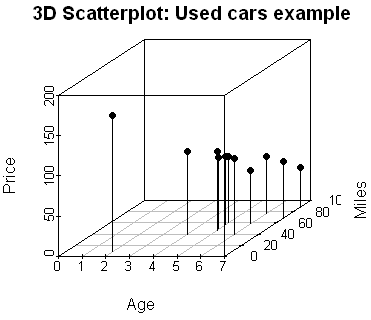
\includegraphics[width=0.4\linewidth,height=0.4\textheight]{figures/3d1} \end{center}

\begin{verbatim}
## Warning in par(usr): argument 1 does not name a graphical parameter

## Warning in par(usr): argument 1 does not name a graphical parameter

## Warning in par(usr): argument 1 does not name a graphical parameter
\end{verbatim}

\begin{center}\includegraphics[width=0.7\linewidth,height=0.7\textheight]{4.4_Regression_Multiple_Regression_Intro_files/figure-latex/unnamed-chunk-2-1} \end{center}

The scatterplot and the correlation matrix show a fairly negative
relationship between the price of the car and both independent variables
(age and miles). It is desirable to have a relationship between each
independent variable and the dependent variable. However, the
scatterplot also shows a positive relationship between the age and the
miles, which isundesirable as it will cause the issue of
Multicollinearity.

\hypertarget{coefficient-of-determination-r2-and-adjusted-r2}{%
\subsection{\texorpdfstring{Coefficient of determination, \(R^2\) and
adjusted
\(R^2\)}{Coefficient of determination, R\^{}2 and adjusted R\^{}2}}\label{coefficient-of-determination-r2-and-adjusted-r2}}

\begin{itemize}
\item
  Recall that, \(R^2\) is a measure of the proportion of the total
  variation in the observed values of the response variable that is
  explained by the multiple linear regression in the \(k\) predictor
  variables \(x_1, x_2, \ldots, x_k\).
\item
  \(R^2\) will increase when an additional predictor variable is added
  to the model. One should not simply select a model with many predictor
  variables because it has the highest \(R^2\) value, it is often good
  to have a model with high \(R^2\) value but only few x's included.
\item
  Adjusted \(R^2\) is a modification of \(R^2\) that takes into account
  the number of predictor variables.
  \[\mbox{Adjusted-}R^2=1-(1-R^2)\frac{n-1}{n-k-1}\]
\end{itemize}

\hypertarget{the-residual-standard-error-s_e}{%
\subsection{\texorpdfstring{The residual standard error,
\(s_e\)}{The residual standard error, s\_e}}\label{the-residual-standard-error-s_e}}

\begin{itemize}
\tightlist
\item
  Recall that,
  \[\text{Residual} = \text{Observed value} - \text{Predicted value.}\]
\end{itemize}

\[e_i=y_i-\hat{y}_i\]

\begin{itemize}
\item
  In a multiple linear regression with \(k\) predictors, the standard
  error of the estimate, \(s_e\), is defined by
  \[s_e=\sqrt{\frac{SSE}{n-(k+1)}}\;\;\;\;\; \text{where}\;\;SSE=\sum (y_i-\hat{y}_i)^2\]
\item
  The standard error of the estimate, \(s_e\), indicates how much, on
  average, the observed values of the response variable differ from the
  predicated values of the response variable. The \(s_e\) is the
  estimate of the common standard deviation \(\sigma\).
\end{itemize}

\hypertarget{inferences-about-a-particular-predictor-variable}{%
\subsection{Inferences about a particular predictor
variable}\label{inferences-about-a-particular-predictor-variable}}

\begin{itemize}
\item
  To test whether a particular predictor variable, say \(x_i\), is
  useful for predicting \(y\) we test the null hypothesis
  \(H_0:\beta_i=0\) against \(H_1:\beta_i\neq 0\).
\item
  The test statistic \[t=\frac{b_i}{s_{b_i}}\] has a \(t\)-distribution
  with degrees of freedom \(df=n-(k+1)\). So we reject \(H_0\), at level
  \(\alpha\), if \(|t|>t_{\alpha/2}.\)
\item
  Rejection of the null hypothesis indicates that \(x_i\) is useful as a
  predictor for \(y\). However, failing to reject the null hypothesis
  suggests that \(x_i\) may not be useful as a predictor of \(y\), so we
  may want to consider removing this variable from the regression
  analysis.
\item
  100(1-\(\alpha\))\% confidence interval for \(\beta_i\) is
  \[b_i \pm t_{\alpha/2} . s_{b_i}\] where \(s_{b_i}\) is the standard
  error of \(b_i\).
\end{itemize}

\begin{center}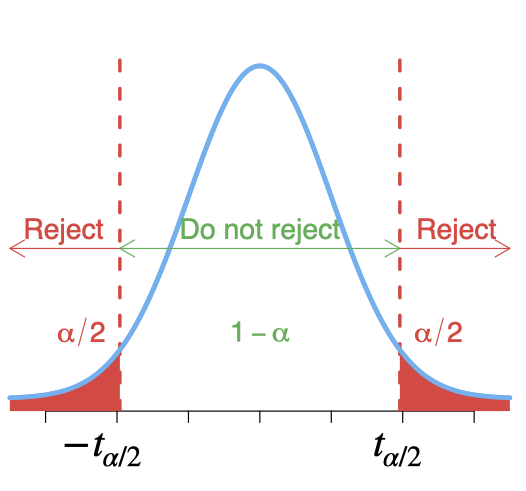
\includegraphics[width=0.3\linewidth,height=0.3\textheight]{figures/Ttest2} \end{center}

\hypertarget{how-useful-is-the-multiple-regression-model}{%
\subsection{How useful is the multiple regression
model?}\label{how-useful-is-the-multiple-regression-model}}

\textbf{Goodness of fit test}

To test how useful is this model, we test the null hypothesis

\(H_0: \beta_1=\beta_2=\ldots =\beta_k=0\), against

\(H_1: \text{at least one of the} \;\beta_i \text{'s is not zero}\). -
The \(F\)-statistic \[F=\frac{MSR}{MSE}=\frac{SSR/k}{SSE/(n-k-1)}\] with
degrees of freedom \(df_1=k\) and \(df_2=n-(k+1)\).

We reject \(H_0\), at level \(\alpha\), if \(F>F_{\alpha}(df_1,df_2)\).

\begin{center}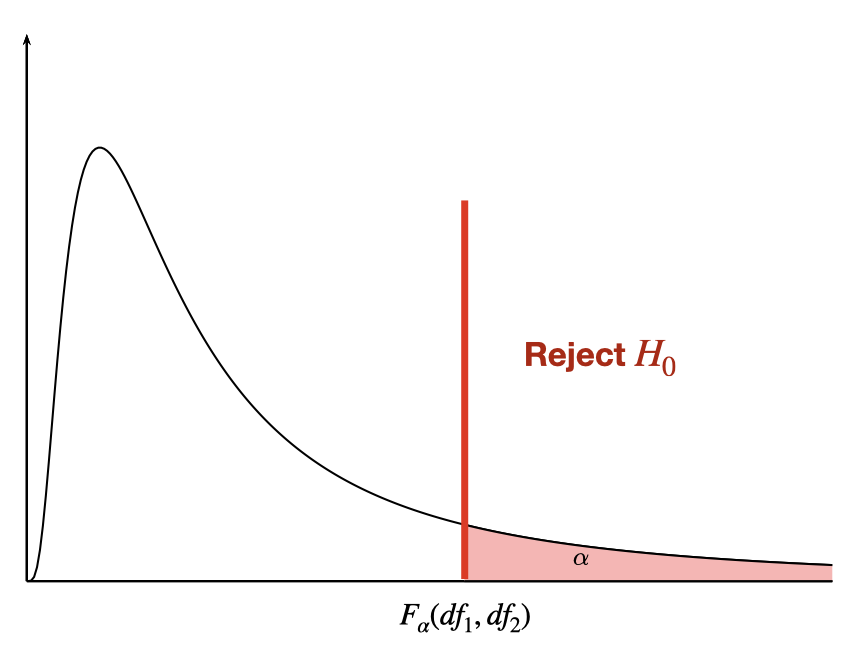
\includegraphics[width=0.4\linewidth,height=0.4\textheight]{figures/Ftest} \end{center}

\hypertarget{used-cars-example-continued}{%
\subsection{Used cars example
continued}\label{used-cars-example-continued}}

Multiple regression equation: \(\hat{y}=183.04-9.50 x_1- 0.82 x_2\)

\begin{center}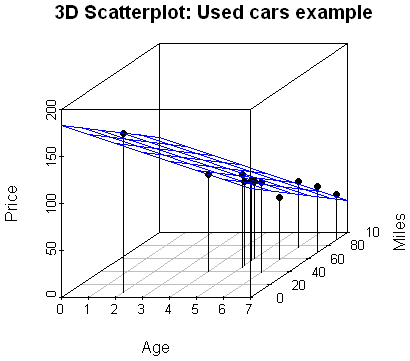
\includegraphics[width=0.4\linewidth,height=0.4\textheight]{figures/3d2} \end{center}

The predicted price for a 4-year-old car that has driven 45 thousands
miles is \[\hat{y}=183.04-9.50 (4)- 0.82 (45)=108.14\] (as units of
\$100 were used, this means \$10814)

\textbf{Extrapolation:} we need to look at the region (all combined
values) not only the range of the observed values of each predictor
variable separately.

\hypertarget{regression-in-r}{%
\subsection{Regression in R}\label{regression-in-r}}

\begin{Shaded}
\begin{Highlighting}[]
\NormalTok{Price}\OtherTok{\textless{}{-}}\FunctionTok{c}\NormalTok{(}\DecValTok{85}\NormalTok{, }\DecValTok{103}\NormalTok{,  }\DecValTok{70}\NormalTok{,  }\DecValTok{82}\NormalTok{,  }\DecValTok{89}\NormalTok{,  }\DecValTok{98}\NormalTok{,  }\DecValTok{66}\NormalTok{,  }\DecValTok{95}\NormalTok{, }\DecValTok{169}\NormalTok{,  }\DecValTok{70}\NormalTok{,  }\DecValTok{48}\NormalTok{)}
\NormalTok{Age}\OtherTok{\textless{}{-}} \FunctionTok{c}\NormalTok{(}\DecValTok{5}\NormalTok{, }\DecValTok{4}\NormalTok{, }\DecValTok{6}\NormalTok{, }\DecValTok{5}\NormalTok{, }\DecValTok{5}\NormalTok{, }\DecValTok{5}\NormalTok{, }\DecValTok{6}\NormalTok{, }\DecValTok{6}\NormalTok{, }\DecValTok{2}\NormalTok{, }\DecValTok{7}\NormalTok{, }\DecValTok{7}\NormalTok{)}
\NormalTok{Miles}\OtherTok{\textless{}{-}}\FunctionTok{c}\NormalTok{(}\DecValTok{57}\NormalTok{,}\DecValTok{40}\NormalTok{,}\DecValTok{77}\NormalTok{,}\DecValTok{60}\NormalTok{,}\DecValTok{49}\NormalTok{,}\DecValTok{47}\NormalTok{,}\DecValTok{58}\NormalTok{,}\DecValTok{39}\NormalTok{,}\DecValTok{8}\NormalTok{,}\DecValTok{69}\NormalTok{,}\DecValTok{89}\NormalTok{)}
\NormalTok{carSales}\OtherTok{\textless{}{-}}\FunctionTok{data.frame}\NormalTok{(}\AttributeTok{Price=}\NormalTok{Price,}\AttributeTok{Age=}\NormalTok{Age,}\AttributeTok{Miles=}\NormalTok{Miles)}


\CommentTok{\# Scatterplot matrix}
\CommentTok{\# Customize upper panel}
\NormalTok{upper.panel}\OtherTok{\textless{}{-}}\ControlFlowTok{function}\NormalTok{(x, y)\{}
  \FunctionTok{points}\NormalTok{(x,y, }\AttributeTok{pch=}\DecValTok{19}\NormalTok{, }\AttributeTok{col=}\DecValTok{4}\NormalTok{)}
\NormalTok{  r }\OtherTok{\textless{}{-}} \FunctionTok{round}\NormalTok{(}\FunctionTok{cor}\NormalTok{(x, y), }\AttributeTok{digits=}\DecValTok{3}\NormalTok{)}
\NormalTok{  txt }\OtherTok{\textless{}{-}} \FunctionTok{paste0}\NormalTok{(}\StringTok{"r = "}\NormalTok{, r)}
\NormalTok{  usr }\OtherTok{\textless{}{-}} \FunctionTok{par}\NormalTok{(}\StringTok{"usr"}\NormalTok{); }\FunctionTok{on.exit}\NormalTok{(}\FunctionTok{par}\NormalTok{(usr))}
  \FunctionTok{par}\NormalTok{(}\AttributeTok{usr =} \FunctionTok{c}\NormalTok{(}\DecValTok{0}\NormalTok{, }\DecValTok{1}\NormalTok{, }\DecValTok{0}\NormalTok{, }\DecValTok{1}\NormalTok{))}
  \FunctionTok{text}\NormalTok{(}\FloatTok{0.5}\NormalTok{, }\FloatTok{0.9}\NormalTok{, txt)}
\NormalTok{\}}
\FunctionTok{pairs}\NormalTok{(carSales, }\AttributeTok{lower.panel =} \ConstantTok{NULL}\NormalTok{, }
      \AttributeTok{upper.panel =}\NormalTok{ upper.panel)}
\end{Highlighting}
\end{Shaded}

\begin{verbatim}
## Warning in par(usr): argument 1 does not name a graphical parameter

## Warning in par(usr): argument 1 does not name a graphical parameter

## Warning in par(usr): argument 1 does not name a graphical parameter
\end{verbatim}

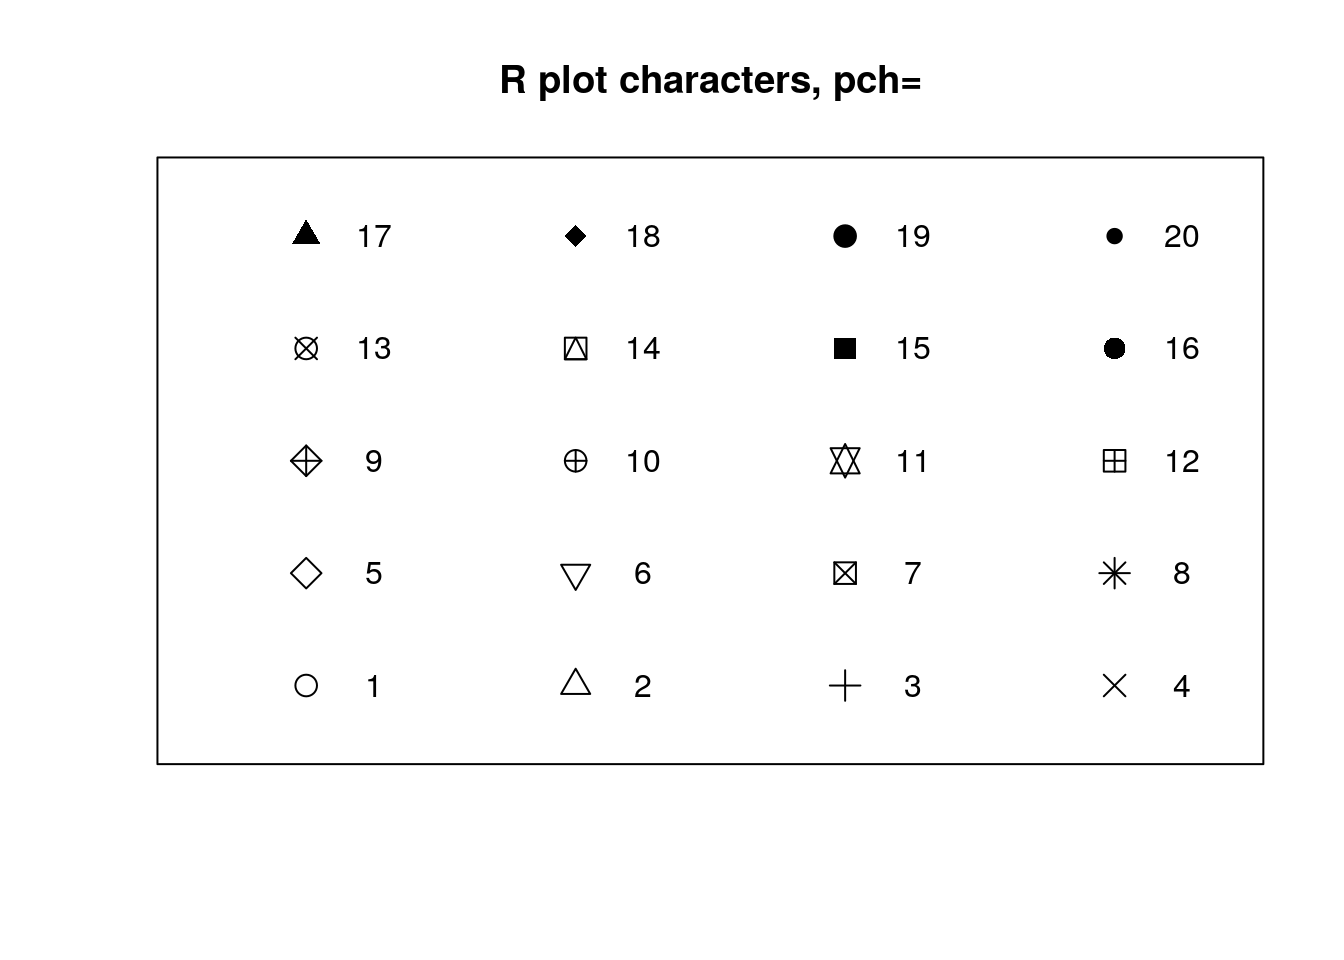
\includegraphics{4.4_Regression_Multiple_Regression_Intro_files/figure-latex/unnamed-chunk-6-1.pdf}

\begin{Shaded}
\begin{Highlighting}[]
\NormalTok{reg }\OtherTok{\textless{}{-}} \FunctionTok{lm}\NormalTok{(Price}\SpecialCharTok{\textasciitilde{}}\NormalTok{Age}\SpecialCharTok{+}\NormalTok{Miles,}\AttributeTok{data=}\NormalTok{carSales)}
\FunctionTok{summary}\NormalTok{(reg)}
\end{Highlighting}
\end{Shaded}

\begin{verbatim}
## 
## Call:
## lm(formula = Price ~ Age + Miles, data = carSales)
## 
## Residuals:
##     Min      1Q  Median      3Q     Max 
## -12.364  -5.243   1.028   5.926  11.545 
## 
## Coefficients:
##             Estimate Std. Error t value Pr(>|t|)    
## (Intercept) 183.0352    11.3476  16.130 2.19e-07 ***
## Age          -9.5043     3.8742  -2.453   0.0397 *  
## Miles        -0.8215     0.2552  -3.219   0.0123 *  
## ---
## Signif. codes:  0 '***' 0.001 '**' 0.01 '*' 0.05 '.' 0.1 ' ' 1
## 
## Residual standard error: 8.805 on 8 degrees of freedom
## Multiple R-squared:  0.9361, Adjusted R-squared:  0.9201 
## F-statistic: 58.61 on 2 and 8 DF,  p-value: 1.666e-05
\end{verbatim}

\begin{Shaded}
\begin{Highlighting}[]
\FunctionTok{confint}\NormalTok{(reg, }\AttributeTok{level=}\FloatTok{0.95}\NormalTok{)}
\end{Highlighting}
\end{Shaded}

\begin{verbatim}
##                  2.5 %      97.5 %
## (Intercept) 156.867552 209.2028630
## Age         -18.438166  -0.5703751
## Miles        -1.409991  -0.2329757
\end{verbatim}

\hypertarget{summary}{%
\subsubsection{Summary}\label{summary}}

\begin{center}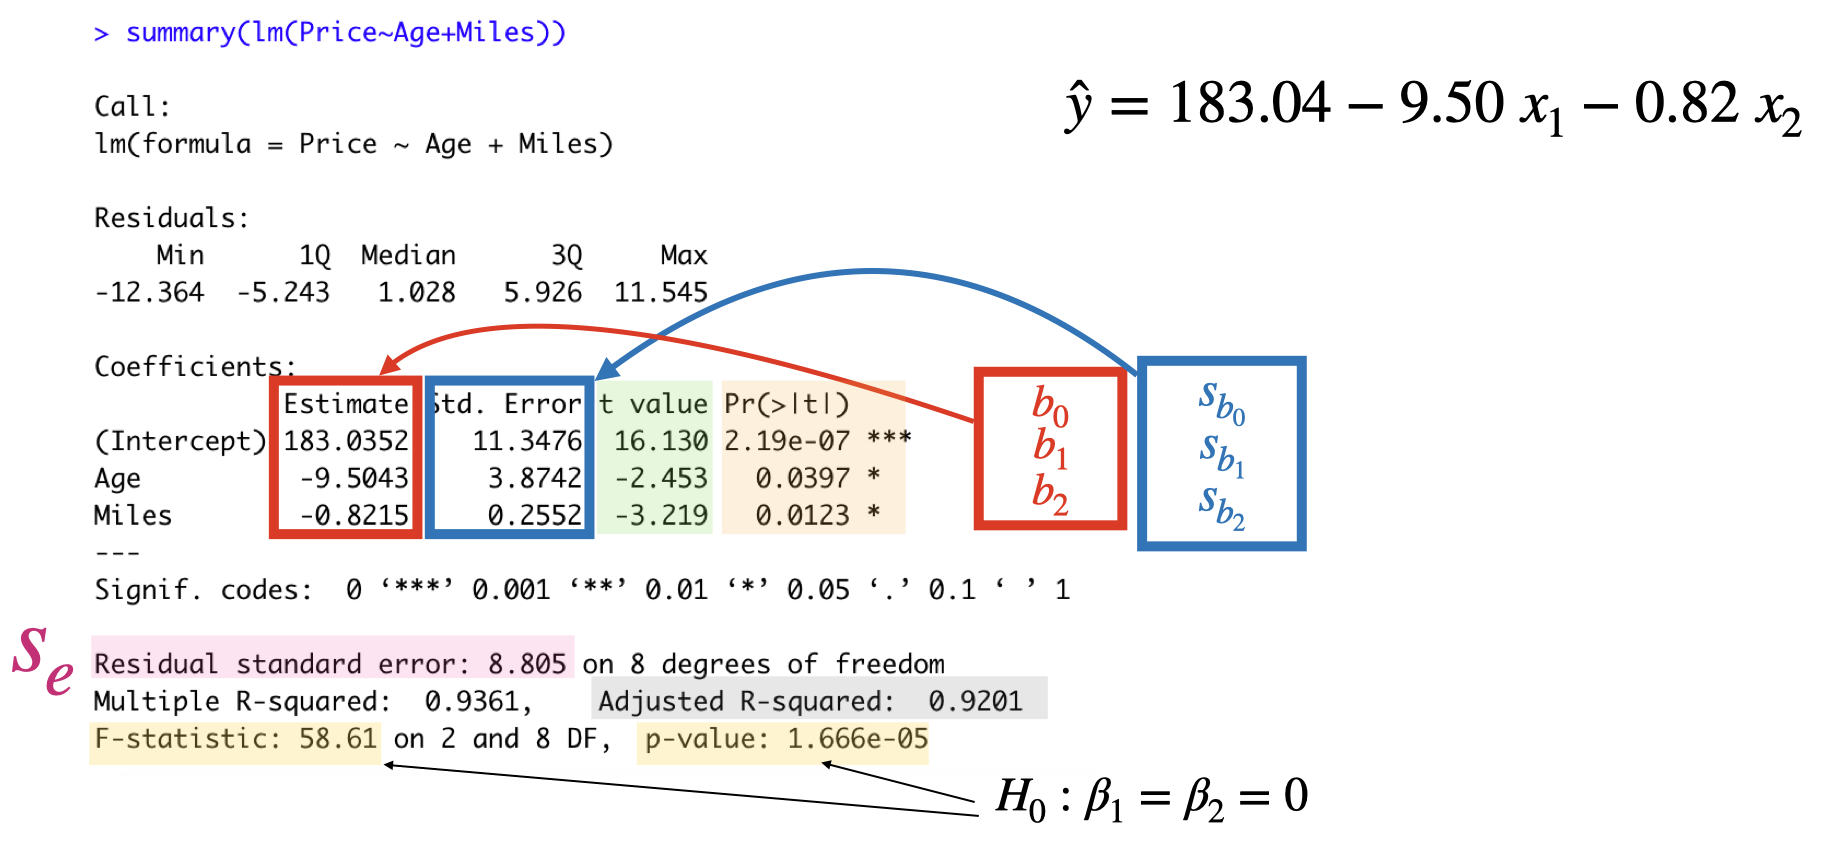
\includegraphics[width=0.6\linewidth,height=0.6\textheight]{figures/Routputmulti} \end{center}

\begin{center}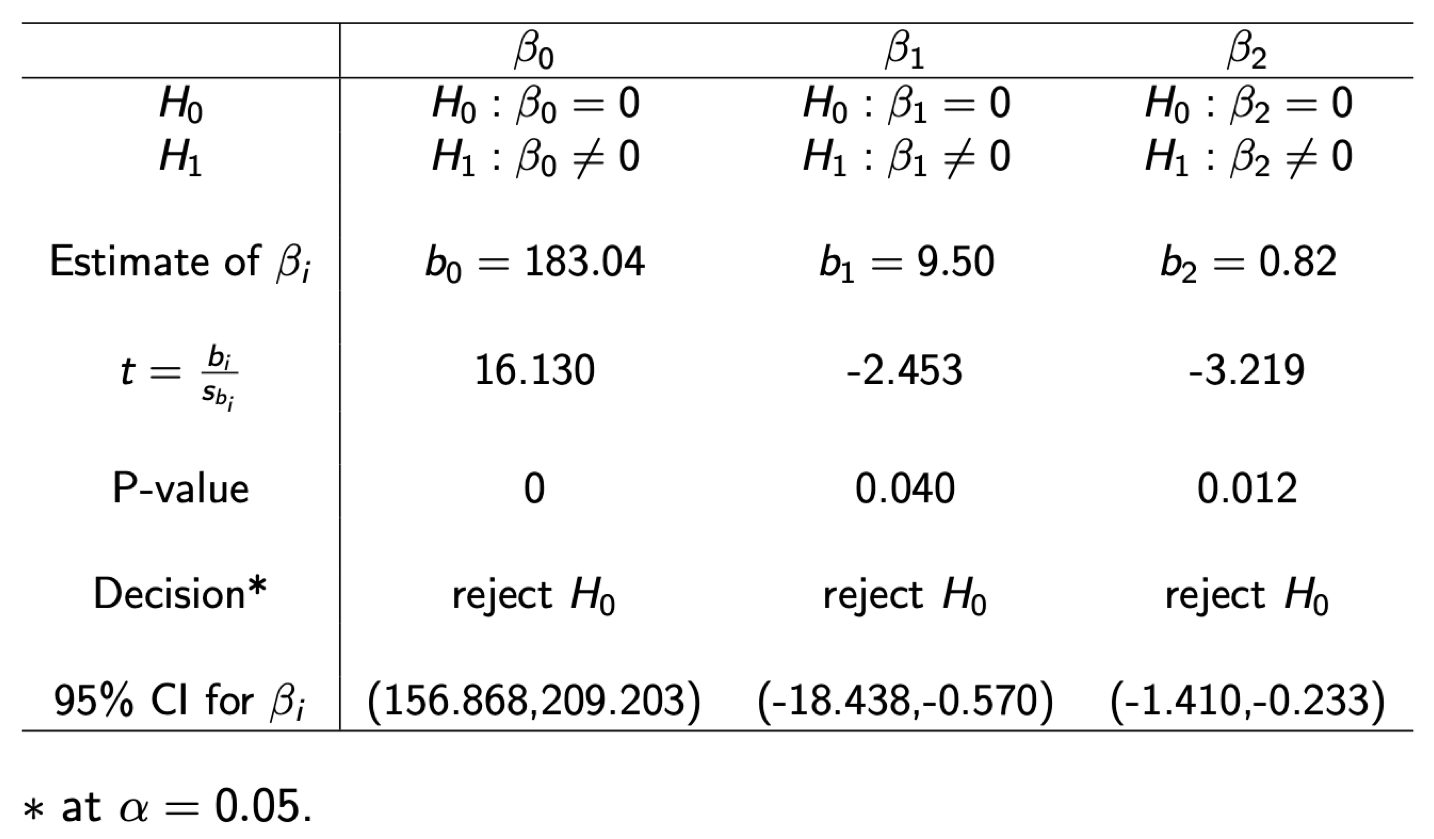
\includegraphics[width=0.6\linewidth,height=0.6\textheight]{figures/Routputmultitable} \end{center}

\hypertarget{multiple-linear-regression-assumptions}{%
\subsection{Multiple Linear Regression
Assumptions}\label{multiple-linear-regression-assumptions}}

\begin{itemize}
\item
  \textbf{Linearity}: For each set of values, \(x_1, x_2, \ldots, x_k\),
  of the predictor variables, the conditional mean of the response
  variable \(y\) is
  \(\beta_0+\beta_1 x_1+\beta_2 x_2+ \ldots+ \beta_k x_k\).
\item
  \textbf{Equal variance (homoscedasticity)}: The conditional variance
  of the response variable are the same (equal to \(\sigma^2\)) for all
  sets of values, \(x_1, x_2, \ldots, x_k\), of the predictor variables.
\item
  \textbf{Independent observations}: The observations of the response
  variable are independent of one another.
\item
  \textbf{Normally}: For each set values, \(x_1, x_2, \ldots, x_k\), of
  the predictor variables, the conditional distribution of the response
  variable is a normal distribution.
\item
  \textbf{No Multicollinearity}: Multicollinearity exists when two or
  more of the predictor variables are highly correlated.
\end{itemize}

\hypertarget{multicollinearity}{%
\subsubsection{Multicollinearity}\label{multicollinearity}}

\begin{itemize}
\item
  Multicollinearity refers to a situation when two or more predictor
  variables in our multiple regression model are highly (linearly)
  correlated.
\item
  The least square estimates will remain unbiased, but unstable.
\item
  The standard errors (of the affected variables) are likely to be high.
\item
  Overall model fit (e.g.~R-square, F, prediction) is not affected.
\end{itemize}

\hypertarget{multicollinearity-detect}{%
\subsubsection{Multicollinearity:
Detect}\label{multicollinearity-detect}}

\begin{itemize}
\item
  Scatterplot Matrix
\item
  \textbf{Variance Inflation Factors}: the Variance Inflation Factors
  (VIF) for the \(i^{th}\) predictor is \[VIF_i=\frac{1}{1-R^2_i}\]
  where \(R^2_i\) is the R-square value obtained by regressing the
  \(i^{th}\) predictor on the other predictor variables.
\item
  \(VIF=1\) indicates that there is no correlation between \(i^{th}\)
  predictor variable and the other predictor variables.
\item
  As rule of thumb if \(VIF>10\) then multicollinearity could be a
  problem.
\end{itemize}

\hypertarget{multicollinearity-how-to-fix}{%
\subsubsection{Multicollinearity: How to
fix?}\label{multicollinearity-how-to-fix}}

\textbf{Ignore:} if the model is going to be used for prediction only.

\textbf{Remove:} e.g.~see if the variables are providing the same
information.

\textbf{Combine:} combining highly correlated variables.

\textbf{Advanced:} e.g.~Principal Components Analysis, Partial Least
Squares.

\(~\)

\hypertarget{regression-in-r-regression-assumptions}{%
\subsection{Regression in R (regression
assumptions)}\label{regression-in-r-regression-assumptions}}

\begin{Shaded}
\begin{Highlighting}[]
\FunctionTok{plot}\NormalTok{(reg, }\AttributeTok{which=}\DecValTok{1}\NormalTok{, }\AttributeTok{pch=}\DecValTok{19}\NormalTok{, }\AttributeTok{col=}\DecValTok{4}\NormalTok{)}
\end{Highlighting}
\end{Shaded}

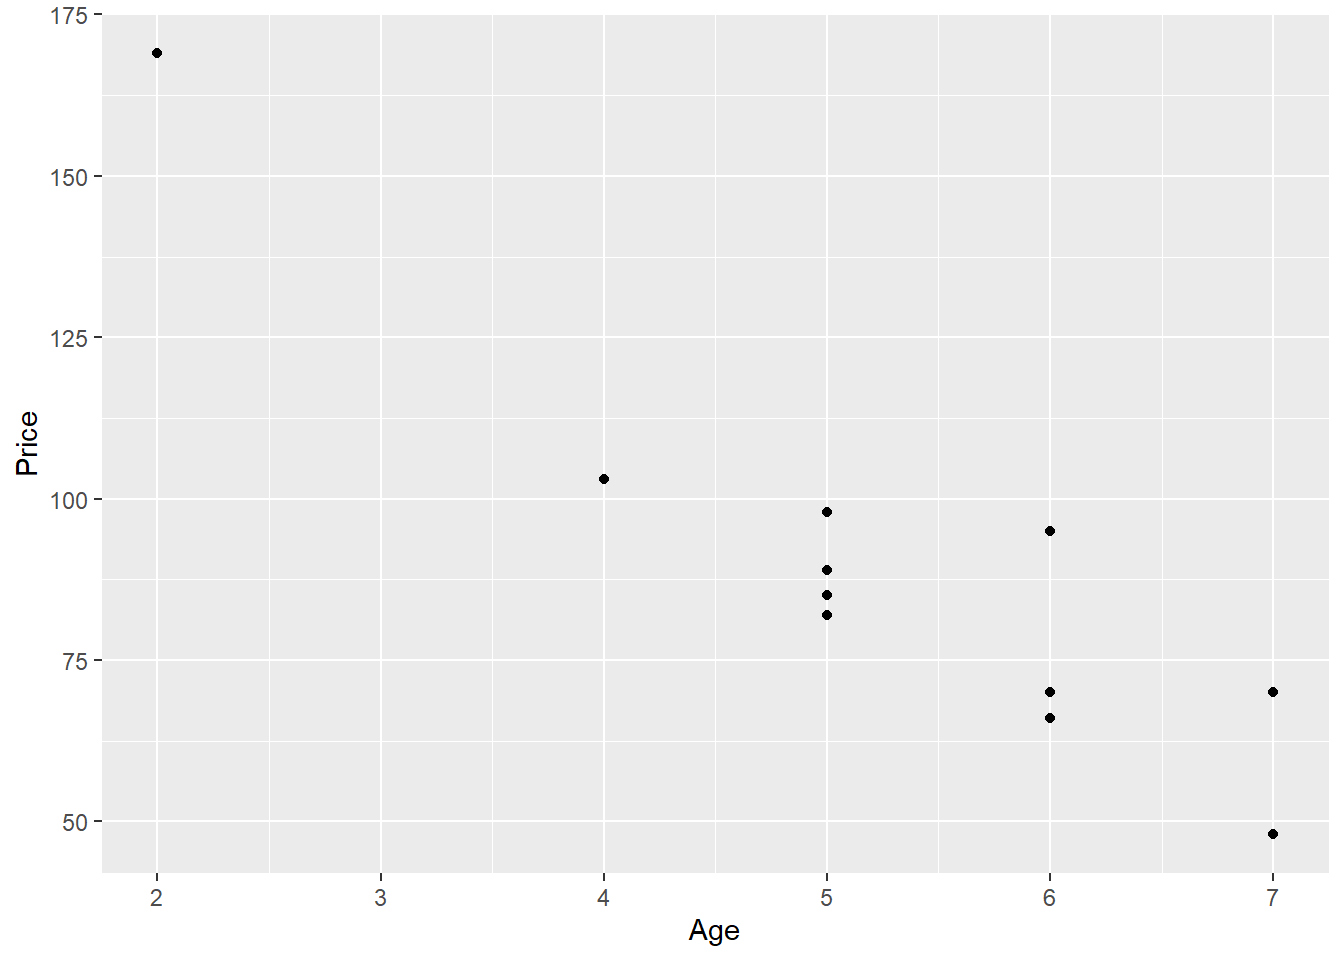
\includegraphics{4.4_Regression_Multiple_Regression_Intro_files/figure-latex/unnamed-chunk-9-1.pdf}

\begin{Shaded}
\begin{Highlighting}[]
\FunctionTok{plot}\NormalTok{(reg, }\AttributeTok{which=}\DecValTok{2}\NormalTok{, }\AttributeTok{pch=}\DecValTok{19}\NormalTok{, }\AttributeTok{col=}\DecValTok{4}\NormalTok{)}
\end{Highlighting}
\end{Shaded}

\includegraphics{4.4_Regression_Multiple_Regression_Intro_files/figure-latex/unnamed-chunk-9-2.pdf}

\begin{Shaded}
\begin{Highlighting}[]
\CommentTok{\# install.packages("car")}
\FunctionTok{library}\NormalTok{(car)}
\end{Highlighting}
\end{Shaded}

\begin{verbatim}
## Loading required package: carData
\end{verbatim}

\begin{Shaded}
\begin{Highlighting}[]
\FunctionTok{vif}\NormalTok{(reg)}
\end{Highlighting}
\end{Shaded}

\begin{verbatim}
##      Age    Miles 
## 3.907129 3.907129
\end{verbatim}

The value of \(VIF=3.91\) indicates a moderate correlation between the
age and the miles in the model, but this is not a major concern.

\end{document}
